\chapter{Fourier and Laplace Transform}
\begin{enumerate}
\item Find the Fourier transform of the function shown in the adjoining figure.
\begin{figure}[H]
	\centering
	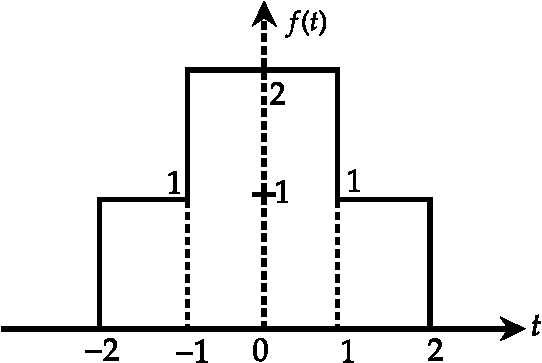
\includegraphics[height=4cm,width=6cm]{CA-01}
\end{figure}
\begin{tasks}(2)
	\task[\textbf{a.}]$\sqrt{\frac{2}{\pi}} \cdot \frac{\sin s}{s}(1-2 \cos s)$
	\task[\textbf{b.}]$\sqrt{\frac{2}{\pi}} \cdot \frac{\cos s}{s}(1-2 \cos s)$
	\task[\textbf{c.}]$\sqrt{\frac{2}{\pi}} \cdot \frac{\sin s}{s}(1+2 \cos s)$
	\task[\textbf{d.}] $\sqrt{\frac{2}{\pi}} \cdot \frac{\cos s}{s}(1+2 \cos s)$
\end{tasks}
\begin{answer}
	$$
	\begin{aligned}
	\text{Here }\quad f(t)&= \begin{cases}2, & \text { for }-1<t<1 \\ 1, & \text { for }-2<t<-1 \\ 1, & \text { for } 1<t<2\end{cases}\\
	\text { The  }&\text{Fourier transform of the function } f(t) \text { is given by }\\
	F[f(t)]&=\frac{1}{\sqrt{2 \pi}} \int_{-\infty}^{\infty} f(t) e^{i s t} d t\\
	\text { Putting} &\text{ the value of }f(t) \text { in }(1), \text { we get }\\
	&=\frac{1}{\sqrt{2 \pi}}\left[\int_{-1}^{1} 2 e^{i s t} d t+\int_{-2}^{-1} 1 \cdot e^{i s t} d t+\int_{1}^{2} 1 \cdot e^{i s t} d t\right]\\
	&=\frac{1}{\sqrt{2 \pi}}\left[2\left(\frac{e^{i s t}}{i s}\right)_{-1}^{1}+\left(\frac{e^{i s t}}{i s}\right)_{-2}^{-1}+\left(\frac{e^{i s t}}{i s}\right)_{1}^{2}\right] \\
	&=\frac{1}{\sqrt{2 \pi}}\left[2\left(\frac{e^{i s}-e^{-i s}}{i s}\right)+\left(\frac{e^{-i s}-e^{-2 i s}}{i s}\right)+\left(\frac{e^{2 i s}-e^{i s}}{i s}\right)\right] \\
	&=\frac{1}{\sqrt{2 \pi }s}\left[2\left(\frac{e^{i s}-e^{-i s}}{i}\right)+\left(\frac{e^{2 i s}-e^{-2 i s}}{i}\right)-\left(\frac{e^{i s}-e^{-i s}}{i}\right)\right]\\&=\frac{1}{\sqrt{2 \pi }s}\left[\left(\frac{e^{i s}-e^{-i s}}{i}\right)+\left(\frac{e^{2 i s}-e^{-2 i s}}{i}\right)\right]\\
	&=\frac{1}{\sqrt{2 \pi }s}[2 \sin s+2 \sin 2 s]=\frac{1}{\sqrt{2 \pi }s}[2 \sin s+4 \sin s \cos s] \\
	&=\frac{2}{\sqrt{2 \pi }s} \sin s(1+2 \cos s)=\sqrt{\frac{2}{\pi}} \cdot \frac{\sin s}{s}(1+2 \cos s)
\end{aligned}
$$
	So the correct answer is \textbf{Option (c)}
\end{answer}
\item Find Fourier Sine transform of $\frac{1}{x}$.
\begin{tasks}(4)
	\task[\textbf{a.}]$\sqrt{\frac{\pi}{2}}$
	\task[\textbf{b.}]$\sqrt{\frac{\pi}{4}}$
	\task[\textbf{c.}]$\sqrt{\frac{3\pi}{2}}$
	\task[\textbf{d.}] $\sqrt{\pi}$
\end{tasks}
\begin{answer}
	$$
	\begin{aligned}
	\text { Here, } f(x)&=\frac{1}{x}\\
	F_{s}[f(x)]&=\sqrt{\frac{2}{\pi}} \int_{0}^{\infty} f(x) \sin s x d x\\
	\text { Putting the value of }& f(x) \text { in }(1) \text {, we get }\\
	F_{s}\left(\frac{1}{x}\right)&=\sqrt{\frac{2}{\pi}} \int_{0}^{\infty} \frac{\sin s x}{x} d x=\sqrt{\frac{2}{\pi}} \int_{0}^{\infty} \frac{\sin \theta}{\frac{\theta}{s}} \frac{d \theta}{s}\\
	\text { Putting s } x&=\theta \text { so that } s d x=d \theta\\
	&=\sqrt{\frac{2}{\pi}} \int_{0}^{\infty} \frac{\sin \theta}{\theta} d \theta=\sqrt{\frac{2}{\pi}}\left(\frac{\pi}{2}\right)\\
	&=\sqrt{\frac{\pi}{2}}
\end{aligned}
$$
	So the correct answer is \textbf{Option (a)}
\end{answer}
\item Find the Fourier Cosine Transform of $f(x)=5 e^{-2 x}+2 e^{-5 x}$
\begin{tasks}(2)
	\task[\textbf{a.}]$10\left(\frac{1}{s^{2}+4}+\frac{1}{s^{2}+25}\right)$
	\task[\textbf{b.}]$10\left(\frac{1}{s^{2}-4}+\frac{1}{s^{2}+25}\right)$
	\task[\textbf{c.}]$10\left(\frac{1}{s^{2}+4}+\frac{1}{s^{2}-25}\right)$
	\task[\textbf{d.}] $10\left(\frac{1}{s^{2}+4}+\frac{1}{s+25}\right)$
\end{tasks}
\begin{answer}
	$$
	\begin{aligned}
	\text { The Fourier } &\text{Cosine Transform of }f(x) \text { is given by }\\
	F_{c}\{f(x)\}&=\sqrt{\frac{2}{\pi}} \int_{0}^{\infty} f(x) \cos s x d x\\
	\text { Putting} &\text{ the value of }f(x) \text { in }(1) \text {, we get } F_{c}\{f(x)\}=\int_{0}^{\infty}\left(5 e^{-2 x}+2 e^{-5 x}\right) \cos s x d x\\
	&=5 \int_{0}^{\infty} e^{-2 x} \cos s x d x+2 \int_{0}^{\infty} e^{-5 x} \cos s x d x \\
	&=5\left[\frac{e^{-2 x}}{(-2)^{2}+s^{2}}(-2 \cos s x+s \sin s x)\right]_{0}^{\infty}+2\left[\frac{e^{-5 x}}{(-5)^{2}+s^{2}}(-5 \cos s x+s \sin s x)\right]_{0}^{\infty}\\
	&=5\left[0-\frac{1}{4+s^{2}}(-2)\right]+2\left[0-\frac{1}{25+s^{2}}(-5)\right]=5\left(\frac{2}{s^{2}+4}\right)+2\left(\frac{5}{s^{2}+25}\right) \\
	&=10\left(\frac{1}{s^{2}+4}+\frac{1}{s^{2}+25}\right)
\end{aligned}
$$
	So the correct answer is \textbf{Option (a)}
\end{answer}
\item Find the Laplace transform of $4 \sin ^{3} t$.
\begin{tasks}(4)
	\task[\textbf{a.}]$\frac{1}{s^{2}+1}-\frac{3}{s^{2}+9}$
	\task[\textbf{b.}]$\frac{3}{s^{2}+1}-\frac{3}{s^{2}+9}$
	\task[\textbf{c.}]$\frac{3}{s^{2}+9}-\frac{3}{s^{2}+3}$
	\task[\textbf{d.}] $\frac{1}{s^{2}+9}-\frac{3}{s^{2}+3}$
\end{tasks}
\begin{answer}
	$$\begin{aligned}
	f(t)&=4 \sin ^{3} t=3 \sin t-\sin 3 t\\
	\because &\left[\sin 3 t=3 \sin t-4 \sin ^{3} \mathrm{t}\right]\\
	\mathrm{L} f(t)&=3 L \sin t-\mathrm{L} \sin 3 t\\&=\frac{3}{s^{2}+1}-\frac{3}{s^{2}+9}
\end{aligned}$$
\end{answer}
\item Find the Laplace transform of the function
$$
f(t)=t e^{-t} \sin 2 t
$$
\begin{tasks}(2)
	\task[\textbf{a.}]$\frac{4(s+1)}{\left[(s+1)^{2}\right]+4}$
	\task[\textbf{b.}]$\frac{4(s+1)}{\left[(s+1)^{2}-4\right]^{2}}$
	\task[\textbf{c.}]$\frac{4(s+1)}{\left[(s-1)^{2}+4\right]^{2}}$
	\task[\textbf{d.}] $\frac{4(s+1)}{\left[(s+1)^{2}+4\right]^{2}}$
\end{tasks}
\begin{answer}
	$$
	\begin{aligned}
	L[\sin 2 t]&=\frac{2}{s^{2}+4}\\
	L\left[e^{-t} \sin 2 t\right]&=\frac{2}{(s+1)^{2}+4}=F(s)\\
	L\left(t e^{-t} \sin 2 t\right)&=-F^{\prime}(s)=-\frac{d}{d s}\left[\frac{2}{(s+1)^{2}+4}\right]=\frac{2 \cdot 2(s+1)}{\left[(s+1)^{2}+4\right]^{2}}=\frac{4(s+1)}{\left[(s+1)^{2}+4\right]^{2}}
\end{aligned}
$$
	So the correct answer is \textbf{Option (d)}
\end{answer}
\item Obtain Laplace transform of rectangular wave given by
\begin{figure}[H]
	\centering
	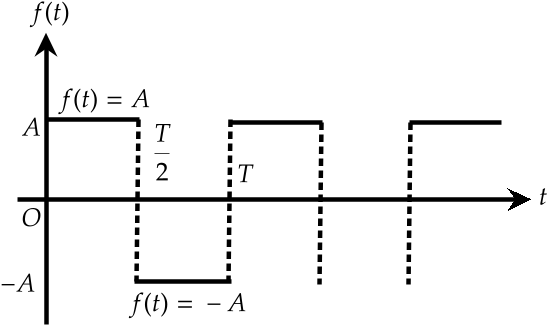
\includegraphics[height=3.9cm,width=6cm]{CA-02}
	 \begin{tasks}(2)
		\task[\textbf{a.}]$\frac{A}{s}\tanh\frac{s\times T}{4}$
		\task[\textbf{b.}]$\frac{A}{s}\tanh\frac{s\times T}{2}$
		\task[\textbf{c.}]$\frac{A}{s}\coth\frac{s\times T}{4}$
		\task[\textbf{d.}] $\frac{A}{s}\tan\frac{s\times T}{4}$
	\end{tasks}
\begin{answer}
	$$
	\begin{aligned}
	\text { We know}&\text{ that Laplace transform of a periodic function i.e., }\\
	L f(t)&=\frac{\int_{0}^{T} e^{-s t} f(t) d t}{1-e^{-s T}}=\frac{\int_{0}^{\frac{T}{2}} e^{-s t} A d t+\int_{\frac{T}{2}}^{T} e^{-s t}(-A) d t}{1-e^{-s T}}\\
	&=A \frac{\left[\frac{e^{-s t}}{-s}\right]_{0}^{\frac{T}{2}}-\left[\frac{e^{-s t}}{-s}\right]_{\frac{T}{2}}^{T}}{1-e^{-s T}}=\frac{A}{1-e^{-s T}}\left[-\frac{e^{-\frac{s T}{2}}}{s}+\frac{1}{s}+\frac{e^{-s T}}{s}-\frac{e^{-\frac{s T}{2}}}{s}\right]\\
	&=\frac{A}{s\left(1-e^{-s T}\right)}\left[1-2 e^{-\frac{s T}{2}}+e^{-s T}\right]=\frac{A}{s\left(1-e^{-s T}\right)}\left[1-e^{-\frac{s T}{2}}\right]^{2}\\
	&=\frac{A\left[1-e^{-\frac{s T}{2}}\right]^{2}}{s\left(1+e^{\frac{-s T}{2}}\right)\left(1-e^{-\frac{s T}{2}}\right)}=\frac{A}{s} \frac{\left(1-e^{-\frac{s T}{2}}\right.}{\left(1+e^{-\frac{s T}{2}}\right)}=\frac{A\left(e^{\frac{s T}{4}}-e^{-\frac{s T}{4}}\right)}{s\left(e^{\frac{s T}{4}}+e^{-\frac{s T}{4}}\right)}=\frac{A}{s} \tanh \frac{s T}{4}
\end{aligned}
$$
	So the correct answer is \textbf{Option (a)}
\end{answer}
\end{figure}
\item Find the inverse Laplace Transform of $\frac{1}{s-2}$
\begin{tasks}(4)
	\task[\textbf{a.}]$e^{t}$
	\task[\textbf{b.}]$e^{t-2}$
	\task[\textbf{c.}]$t$
	\task[\textbf{d.}] $e^{2 t}$
\end{tasks}
\begin{answer}
	$$
	\begin{aligned}
	L^{-1}\left\lbrace  \frac{1}{s-2}\right\rbrace &=e^{2 t}
\end{aligned}
$$
	So the correct answer is \textbf{Option (d)}
\end{answer}
\item If $f(x)=\left\{\begin{array}{ll}0 & \text { for } x<3, \\ x-3 & \text { for } x \geq 3\end{array}\right.$ then the Laplace transform of $f(x)$ is
\begin{tasks}(4)
	\task[\textbf{A.}] $s^{-2} e^{3 s}$
	\task[\textbf{B.}] $s^{2} e^{3 s}$
	\task[\textbf{C.}] $s^{-2}$
	\task[\textbf{D.}] $s^{-2} e^{-3 s}$
\end{tasks}
\begin{answer}
	$$
	\begin{aligned}
	L\{f(x)\}&=\int_{0}^{\infty} e^{-s x} f(x) d x\\&=\int_{0}^{3} e^{-s x} f(x) d x+\int_{3}^{\infty} e^{-s x} f(x) d x\\&=\int_{3}^{\infty}(x-3) e^{-s x} d x\\
	L\{f(x)\}&=\left.(x-3) \frac{e^{-s x}}{-s}\right|_{3} ^{\infty}-\int_{3}^{\infty} 1 \cdot\left(\frac{e^{-s x}}{-s}\right) d x\\&=0+\frac{1}{s} \int_{3}^{\infty} e^{-s x} d x\\&=\frac{1}{s}\left[\frac{e^{-s x}}{-s}\right]_{3}^{\infty}=s^{-2} e^{-3 s}
	\end{aligned}
$$
	So the correct answer is \textbf{Option (D)}
\end{answer}
\item The graph of the function $f(x)=\left\{\begin{array}{ll}1 & \text { for } 2 n \leq x \leq 2 n+1 \\ 0 & \text { for } 2 n+1 \leq x \leq 2 n+2\end{array}\right.$ where $n=(0,1,2, \ldots \ldots)$ is shown below. Its Laplace transform $\tilde{f}(s)$ is
\begin{figure}[H]
	\centering
	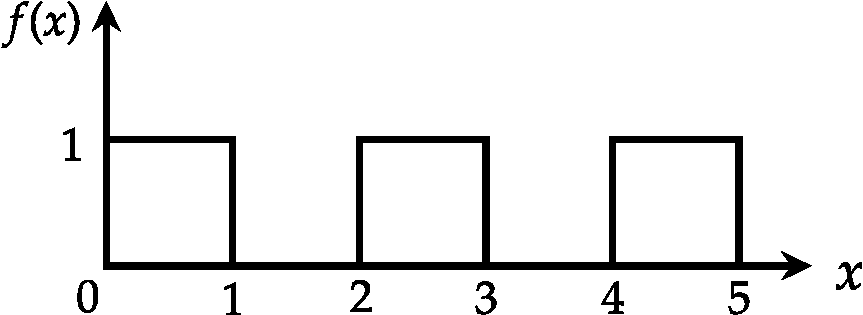
\includegraphics[height=2.7cm,width=7.5cm]{CA-03}
\end{figure}
\begin{tasks}(4)
	\task[\textbf{A.}] $\frac{1+e^{-s}}{s}$
	\task[\textbf{B.}] $\frac{1-e^{-s}}{s}$
	\task[\textbf{C.}] $\frac{1}{s\left(1+e^{-s}\right)}$
	\task[\textbf{D.}]  $\frac{1}{s\left(1-e^{-s}\right)}$
\end{tasks}
\begin{answer}
	$$
	\begin{aligned}
	L(f(x))&=\int_{0}^{\infty} e^{-s x} f(x) d x\\&=\int_{0}^{1} e^{-s x} \cdot 1 d x+\int_{1}^{2} e^{-s x} \cdot 0 d x+\int_{2}^{3} e^{-s x} \cdot 1 d x+\ldots \ldots\\
	&=\left[\frac{e^{-s x}}{-s}\right]_{0}^{1}+0+\left[\frac{e^{-s x}}{-s}\right]_{2}^{3}+\ldots \ldots\\&=\frac{1}{-s}\left[e^{-s}-1\right]+\frac{1}{-s}\left[e^{-3 s}-e^{-2 s}\right]+\ldots \ldots\\
	&=\frac{1}{-s}\left[-1+e^{-s}-e^{-2 s}+e^{-3 s}+\ldots \ldots . .\right]\\&=\frac{1}{s}\left[1-e^{-s}+e^{-2 s}-e^{-3 s}+\ldots .\right]\\
	\text{Since }S_{\infty}&=\frac{a}{1-r}\text{ where }r=-e^{-s}\text{ and }a\\&=1 \Rightarrow S_{\infty}=\frac{1}{s}\left[\frac{1}{\left(1+e^{-s}\right)}\right]
	\end{aligned}
	$$
		So the correct answer is \textbf{Option (c)}
\end{answer}
\item The Fourier transform $\int_{-\infty}^{\infty} d x f(x) e^{i k x}$ of the function $f(x)=e^{-|x|}$
\begin{tasks}(4)
	\task[\textbf{A.}] $-\frac{2}{1+k^{2}}$
	\task[\textbf{B.}] $-\frac{1}{2\left(1+k^{2}\right)}$
	\task[\textbf{C.}] $\frac{2}{1+k^{2}}$
	\task[\textbf{D.}] $\frac{2}{\left(2+k^{2}\right)}$
\end{tasks}
\begin{answer}
	$$
	\begin{aligned}
\int_{-\infty}^{+\infty} d x e^{-|x|} e^{i k x}&=\int_{-\infty}^{+\infty} d x e^{-|x|} \cos k x d x\text{ odd functions in }k x\text{ vanishes}\\
\Rightarrow 2 \int_{0}^{\infty} e^{-x} \cos k x d x&=2 \frac{e^{-x}}{1+k^{2}}[-\cos k x+k \sin k x]_{0}^{\infty}\\
\because \int e^{a x} \cos b x d x&=\frac{e^{a x}}{a^{2}+b^{2}}[a \cos b x+b \sin b x]\\
\Rightarrow 2 \int_{0}^{\infty} e^{-x} \cos k x d x&=2 \frac{e^{0}}{1+k^{2}}=\frac{2}{1+k^{2}}
\end{aligned}
$$
So the correct answer is \textbf{Option (C)}
\end{answer}
\item Consider the differential equation $\frac{d y}{d t}+a y=e^{-b t}$ with the initial condition $y(0)=0$. Then the Laplace transform $Y(s)$ of the solution $y(t)$ is
\begin{tasks}(4)
	\task[\textbf{A.}] $\frac{1}{(s+a)(s+b)}$
	\task[\textbf{B.}] $\frac{1}{b(s+a)}$
	\task[\textbf{C.}] $\frac{1}{a(s+b)}$
	\task[\textbf{D.}] $\frac{e^{-a}-e^{-b}}{b-a}$
\end{tasks}
\begin{answer}
	$$
	\begin{aligned}
	\text{Given }\frac{d y}{d t}+a y&=e^{-b t}\\
	\text{Taking }&\text{Laplace transform of both sides}\\
	\text{	We obtain}\\
	L\left\{\frac{d y}{d t}\right\}+a L\{y(t)\}&=L\left\{e^{-b t}\right\} \Rightarrow s Y(s)-y(0)+a Y(s)=\frac{1}{s+b}\\
	\text{Since, }	y(0)&=0,\text{ we obtain}\\
	(s+a) Y(s)&=\frac{1}{s+b} \Rightarrow Y(s)=\frac{1}{(s+a)(s+b)}
	\end{aligned}
	$$
	So the correct answer is \textbf{Option (A)}
\end{answer}
\item The Laplace transformation of $e^{-2 t} \sin 4 t$ is
\begin{tasks}(2)
	\task[\textbf{a.}]$\frac{4}{s^{2}+4 s+25}$
	\task[\textbf{b.}]$\frac{4}{s^{2}+4 s+20}$
	\task[\textbf{c.}]$\frac{4 s}{s^{2}+4 s+20}$
	\task[\textbf{d.}] $\frac{4 s}{2 s^{2}+4 s+20}$
\end{tasks}
\begin{answer}
	$$\begin{aligned}
	\because L\left[e^{-a t} \sin b t\right]&=\frac{b}{(s+a)^{2}+b^{2}}\\
	\Rightarrow L\left[e^{-2 t} \sin 4 t\right]&=\frac{4}{(s+2)^{2}+4^{2}}\\&=\frac{4}{s^{2}+4 s+20}
	\end{aligned}$$
	Correct option is (C)
\end{answer}
\item The Fourier transform of the function $\frac{1}{x^{4}+3 x^{2}+2}$ up to proportionality constant is
\begin{tasks}(1)
	\task[\textbf{a.}] $\sqrt{2} \exp \left(-k^{2}\right)-\exp \left(-2 k^{2}\right)$
	\task[\textbf{b.}]$\sqrt{2} \exp (-|k|)-\exp (-\sqrt{2}|k|)$
	\task[\textbf{c.}]$\sqrt{2} \exp (-\sqrt{|k|})-\exp (-\sqrt{2|k|})$
	\task[\textbf{d.}] $\sqrt{2} \exp \left(-\sqrt{2} k^{2}\right)-\exp \left(-2 k^{2}\right)$
\end{tasks}
\begin{answer}
	$$\begin{aligned}
	f(x)&=\frac{1}{\left(x^{4}+3 x^{2}+2\right)}=\frac{1}{\left(x^{2}+1\right)}-\frac{1}{\left[x^{2}+(\sqrt{2})^{2}\right]}\\
	\text{Now, Fourier transform}&\text{ of f(x) is,}\\
	F(p)&=A \int_{-\infty}^{\infty} f(x) e^{-1 k x} d x\\
	&=A \int_{-\infty}^{\infty}\left[\frac{1}{\left(x^{2}+1\right)}-\frac{1}{x^{2}+(\sqrt{2})^{2}}\right] e^{-i k x} d x\\&=A\left[\int_{-\infty}^{\infty} \frac{1}{\left(x^{2}+1\right)} \times e^{-i k x} d x-\int_{-\infty}^{\infty} \frac{e^{-i k x}}{x^{2}+(\sqrt{2})^{2}} d x\right]\\
	\because \int_{-\infty}^{\infty} \frac{1}{\left(x^{2}+a^{2}\right)} e^{-i k x} d x&=\sqrt{\frac{\pi}{2}} \frac{e^{-a|k|}}{a}\\
	F(k)&=A\left[\sqrt{\frac{\pi}{2}} \frac{e^{-|k|}}{1}-\sqrt{\frac{\pi}{2}} \frac{e^{-\sqrt{2}|k|}}{\sqrt{2}}\right]\\&=\frac{A \sqrt{\pi}}{2}[\sqrt{2} \exp (-|k|)-\exp (-\sqrt{2}|k|)]
	\end{aligned}$$
	Correct option is (A)
\end{answer}
\item The Laplace transform of $\frac{(\sin (a t)-a t \cos (a t))}{\left(2 a^{3}\right)}$ is
\begin{tasks}(4)
	\task[\textbf{a.}]$\frac{2 a s}{\left(s^{2}+a^{2}\right)^{2}}$
	\task[\textbf{b.}]$\frac{s^{2}-a^{2}}{\left(s^{2}+a^{2}\right)^{2}}$
	\task[\textbf{c.}] $\frac{1}{(s+a)^{2}}$
	\task[\textbf{d.}] $\frac{1}{\left(s^{2}+a^{2}\right)^{2}}$
\end{tasks}
\begin{answer}
	$$\begin{aligned}
	L\left\{\frac{\sin a t-a t \cos a t}{2 a^{3}}\right\}=\frac{1}{\left(s^{2}+a^{2}\right)^{2}}
	\end{aligned}$$
	
	Correct option is (D)
\end{answer}
\item Find the solution to the following ordinary differential equation (ODE) using Laplace transform method.
$y^{\prime \prime}-5 y^{\prime}+6 y=0$ given that $y(0)=2$ and $y^{\prime}(0)=2$
\begin{tasks}(2)
	\task[\textbf{a.}] $y(t)=4 e^{2 t}+2 e^{3 t}$
	\task[\textbf{b.}]$y(t)=4 e^{3 t}+2 e^{2 t}$
	\task[\textbf{c.}]$y(t)=4 e^{2 t}-2 e^{3 t}$
	\task[\textbf{d.}] None of these 
\end{tasks}

\begin{answer}
	Taking Laplace transform on both sides of the given differential equation, we get
	$$
	\begin{aligned}
	&\left[s^{2} Y(s)-s y(0)-y^{\prime}(0)\right]-5[s Y(s)-y(0)+6 Y(s)=0\\
	\text{Substituting}&\text{ the initial conditions, we get }\\
	&\left(s^{2} Y(s)-2 s-2\right)-5(s Y(s)-2)+6 Y(s)=0\\
&	Y(s)\left(s^{2}-5 s+6\right)-2 s+8=0\\
\Rightarrow Y(s)=\frac{2 s-8}{\left(s^{2}-5 s+6\right)}&=\frac{2 s-8}{(s-2)(s-3)}\\
\text{ Using  }&\text{partial fraction expansion, we get}\\
Y(s)=\frac{4}{s-2}-\frac{2}{s-3}\\
\text { Taking }&\text{inverse Laplace transform, we get }\\
y(t)&=4 e^{2 t}-2 e^{3 t}
\end{aligned}
$$
	So the correct answer is \textbf{Option (c)}
\end{answer}
	
	
	
	
	
	
	
	
	
	
	
\end{enumerate}